\documentclass[11pt]{exam}
\usepackage[margin=1in]{geometry}
\pagestyle{plain}
\usepackage{amsmath,amsfonts,amssymb,amsthm,enumerate}
\usepackage{multicol}
\usepackage[]{graphicx}
\usepackage{hyperref}
\usepackage{tikz}
\usepackage{pgfplots}
\usepackage{subfigure}
\usepackage[final]{pdfpages}

\addtolength{\footskip}{2\baselineskip} % to lower the page numbers
\title{\vspace{-0.5in} Math 115 \\ Worksheet Section 4.3}
\date{}


% \theoremstyle{definition}
% \newtheorem{problem}{Problem}
\renewcommand{\questionlabel}{\textbf{Problem~\thequestion.}}
%\printanswers

\begin{document}
\maketitle
\vspace{-0.75in}
\section*{Optimization questions: what to do?}


\noindent
Read the problem carefully:
\begin{itemize}
\item What is the quantity to be optimized? 
\item What information is given?
\item Draw a picture that helps you organize the information given.
\item Introduce variables to label the information given to you.
\item What formulas are available that could be useful?
\item Write a function for the quantity you will optimize using your formulas. 
\item Determine the domain of your function.
\item Use what you learned in sections 4.1 and 4.2 to find your answer(s).
\end{itemize}
\begin{questions}
\question City council is planning to construct a new sports ground in the shape of a
rectangle with semicircular ends. A running track 400 meters long is to go around
the perimeter.
\begin{parts}
\part What choice of dimensions will make the rectangular area in the
  center as large as possible?
  \vspace{0.4in}
\part What dimensions would maximize the total area
enclosed by the running track?
  \vspace{0.4in}
\end{parts}
\begin{solution}
  Let \(r\) be the radius of the half circles and \(x\) be the
  side length of the rectangle (so our rectangle is \(x\) by \(2r\)). 
  \begin{enumerate}[(a)]
  \item We first observe that the quantity to be optimized is the area
    of the rectangular area and it is
    given by \[
      A = 2rx \,.
    \]
    We also note that the running track has length \(P = 2x + 2\pi
    r\) since it is the perimeter of this shape and
    \(P=400\). Thus, \(r = \frac{400-2x}{2\pi} =
    \frac{200-x}{\pi}\). We substitute this back into our area
    equation to get a function in terms of \(x\):\[
      A(x) = \frac{400x-2x^2}{\pi}
    \]
    We determine that the domain is \(0 \leq x \leq 200\), since any
    values outside of this would give nonsensical answers. (We cannot
    have negative length and if \(x > 200\), we would get a negative
    value for \(r\).) Now, we can use our method for finding global
    extrema for continuous functions on a closed interval.

    We compute \(A'(x) = \frac{400}{\pi}-\frac{4}{\pi}x\). Then, we check
    \begin{itemize}
    \item \(A'(x) = 0\): at \(x=100\)
    \item \(A'(x)\) DNE: none
    \end{itemize}
    Then, we check our end points and critical point \[
      \begin{array}{|c|c|}
        \hline
        x & A(x)\\
        \hline
        0 & 0\\
        \hline
        100 & \frac{20000}{\pi}\\
        \hline
        200 & 0\\
        \hline
      \end{array}
    \]
    Thus, \(x=100\) gives a global maximum of \(A(x)\). Therefore, the
    dimensions of \(x=100\) meters and \(r = \frac{100}{\pi}\) meters maximizes the area.
  \item Using the same variable names as above for \(r,x\), the total
    area enclosed is given by \[
      A = 2rx + \pi r^2
    \]
    We still have \(400 = 2x + 2\pi r\), but it is easier to put \(2x
    = 400 - 2\pi r\) and substitute into our equation for \(A\) to
    get \[
      A(r) = r(400-2\pi r) + \pi r^2 = 400r-\pi r^2
    \]
    Our function \(A(r)\) has domain \(0 \leq r \leq
    \frac{200}{\pi}\) for similar reasons as part (a). Thus, we can
    use our method for finding global extrema for continuous functions
    on a closed interval.

    We compute \(A'(r) = 400-2\pi r\). Then, we check
    \begin{itemize}
    \item \(A'(r) = 0\): at \(r = \frac{200}{\pi}\)
    \item \(A'(r)\) DNE: none
    \end{itemize}
    Then, we check our end points and critical point (which is an
    endpoint) \[
   \begin{array}{|c|c|}
        \hline
        r & A(r)\\
        \hline
        0 & 0\\
        \hline
        \frac{200}{\pi} & \frac{40000}{\pi}\\
        \hline
      \end{array}
    \]
    So, setting \(r = \frac{200}{\pi}\) meters and \(x = 0\) meters
    (resulting in a circular track) maximizes the area enclosed by the track.
  \end{enumerate}
\end{solution}
\question The sum of two positive numbers is 48. What is the smallest possible value of the sum of their squares?
  \begin{solution}
    Let our two numbers be \(x\) and \(y\). The question tells us that
    \(x+y=48\) and we want to minimize the sum \(S\) given by \[
      S = x^2+y^2
    \]
    To do this, we set \(y = 48-x\) to get a function of \(x\) \[
      S(x) = x^2 + (48-x)^2 = x^2 + 48^2 - 96x + x^2 = 2x^2-96x+48^2
    \]
    Here, the domain is \(0 < x < 48\) since \(x,y\) must both be
    positive numbers (\(0\) is not positive).

    Now, we differentiate to
    get \(S'(x) = 4x-96\). Then, we check
    \begin{itemize}
    \item \(S'(x) = 0\): at \(x = 24\)
    \item \(S'(x)\) DNE: none
    \end{itemize}
    Thus, we have one critical point on an open interval, \((0,48)\),
    so we can use the first derivative test to check:
    \begin{itemize}
    \item Test point \(S'(1) = -92\)
    \item Test point \(S'(42) = 72\)
    \end{itemize}
    \(\implies\)
    \begin{tikzpicture}
      \node at (-1,0) {$S'$};
      \draw (0,0)--(4,0);
      \draw (2,-.1)--(2,.1);
      \node at (2,-.4) {$24$};
      \node at (1,.2) {$-$};
      \node at (3,.2) {$+$};
    \end{tikzpicture}

  Thus, since \(x=24\) is a local minimum and the only critical point
  on an open interval, it must be a global minimum. Therefore,
  \(24^2+24^2 = 1152\) is the smallest possible value of the sum of
  the squares of \(x,y\).

  Note, since \(x=24, y=24\) is a global minimum and \(S(x)\) is
  continuous, there would not have been any harm in extending our
  domain to include \(x=0\) and \(x=48\) and using the closed interval
  method for the purposes of finding a global minimum, but it would
  have led us astray if we had been asked for a global maximum.
  \end{solution}
  \vspace{0.4in}
\question  A factory makes cylindrical cans of volume 500 cubic centimeters.  Suppose the metal for the sides of the can costs 1 cent per cm$^2$, and the metal for the top and the bottom costs twice as much.  Find the dimensions of the can that minimizes its cost.
  \begin{solution}
    Recall the volume of a cylinder is \(V = \pi r^2 h\) for radius
    \(r\) and height \(h\). Furthermore, surface area \(S = 2\pi r h +
    2 \pi r^2\).  Therefore, the cost, \(C\), of producing such a can is \[
      C = 1 \cdot 2 \pi r h + 2 \cdot 2 \pi r^2 = 2 \pi r h + 4 \pi r^2
    \]
    To make this a function of \(r\), we can use the fact that \(V =
    500\) cm\({}^3\) to solve \(h = \frac{500}{\pi r^2}\). Plugging
    this into \(C\), we get \[
      C(r) = 2 \pi r \left( \frac{500}{\pi r^2} \right) + 4 \pi r^2 =
      1000 r^{-1} + 4 \pi r^2
    \]
    The domain of this problem is \(0 < r < \infty\) since \(r\)
    cannot be negative, nor can it be \(0\), since then we could not
    have \(V = 500\).

    Now, we differentiate to get \(C'(r) = -1000r^{-2} + 8\pi
    r\). Then, we check 
    \begin{itemize}
    \item \(C'(r) = 0\): at \(r = \left(\frac{1000}{8\pi}\right)^{1/3} =
      5 \pi^{-1/3}\)
    \item \(C'(r)\) DNE: at \(r = 0\), but not in the domain.
    \end{itemize}
    Thus, since we have one critical point in the open interval
    \((0,\infty)\), we can use the first derivative test to check:
    \begin{itemize}
    \item \(C'(1) = -1000+8\pi < 0\)
    \item \(C'(100) = -0.1+800\pi > 0\)
    \end{itemize}
    \(\implies\)
    \begin{tikzpicture}
      \node at (-1,0) {$C'$};
      \draw (0,0)--(4,0);
      \draw (2,-.1)--(2,.1);
      \node at (2,-.4) {$5\pi^{-1/3}$};
      \node at (1,.2) {$-$};
      \node at (3,.2) {$+$};
    \end{tikzpicture}

    Thus, since \(r = 5 \pi^{-1/3}\) is a local minimum and the only
    critical point on an open interval, it must be a global
    minimum. Therefore, a can with radius \(5 \pi^{-1/3}\) cm and
    height \(\frac{500}{25 \pi^{1-2/3}} = 20 \pi^{-1/3}\) cm will
    minimize the cost.
  \end{solution}
  \vspace{0.4in}
\question  A wire six meters long is cut into 12 pieces. These pieces are welded together at
right angles to form the frame of a box with square base. Where should the cuts
be made to maximize the total surface area of the box?
\begin{solution}
  Let \(x\) be the side length of the square base and let \(y\) be the
  height of the box frame. Then, the surface area of the box is given
  by \[
    S = 2x^2 + 4xy
  \]
  and we know that \(8x+4y = 6\) from the fact that all the pieces
  come from \(6\) meters of wire. Thus, we have that \(y =
  \frac{6-8x}{4} = \frac{3-4x}{2}\). Substituting this into \(S\), we
  get \[
    S(x) = 2x^2 + 4x\left( \frac{3-4x}{2} \right) = 2x^2 + 6x - 8x^2 = -6x^2+6x
  \]
  with domain \(0 < x < \frac{3}{4}\). Note the end points are not
  included, otherwise we would not be able to have \(12\) pieces of
  wire.

  Now, we differentiate to get \(S'(x) = -12x+6\). Then, we check
  \begin{itemize}
  \item \(S'(x) = 0\): at \(x = \frac{1}{2}\)
  \item \(S'(x)\) DNE: none
  \end{itemize}
  Thus, since we have one critical point on an open interval, we can
  use the first derivative test to check test points
  \begin{itemize}
  \item \(S'(0.25) = 2\)
  \item \(S'(\frac{7}{12}) = -1\)
  \end{itemize}
    \(\implies\)
    \begin{tikzpicture}
      \node at (-1,0) {$S'$};
      \draw (0,0)--(4,0);
      \draw (2,-.1)--(2,.1);
      \node at (2,-.4) {$\frac{1}{2}$};
      \node at (1,.2) {$+$};
      \node at (3,.2) {$-$};
    \end{tikzpicture}

    Thus, since \(x = \frac{1}{2}\) is a local maximum and the only
    critical point on an open interval, it must be a global
    maximum. Therefore, such a box assembled with dimensions
    \(\frac{1}{2} \text{ meters} \times \frac{1}{2} \text{ meters}
    \times \frac{1}{2} \text{ meters}\) will maximize the total
    surface area. In other words, the cuts should be made every half meter.
\end{solution}
\pagebreak
\question (Fall 2013 Exam 2) % problem 1
Liam wants to build a 1600 square foot, rectangular swimming pool behind his new house. He also wants 8-foot wide decks on two sides of the pool
and 10-foot wide decks on the other two sides of the pool (see the diagram below).
\begin{center}
	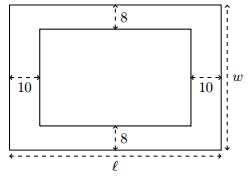
\includegraphics[width=2in]{pool.jpg}
\end{center}

\begin{enumerate}[(a)]
	
	\item  Let $\ell$ and $w$ be the length and width (in feet) of the pool area including the
	decks as shown in the diagram. Write a formula for $\ell$ in terms of $w$.
	
	
	\item  Write a formula for the function $A(w)$ which gives the total area (in square
	feet) of the pool and the decks in terms of only the width $w$. Your formula should not
	include the variable $\ell$.   (This is the function Liam would minimize in order to find the
	minimum area that his pool and deck will take up in his yard. You do not need to do the
	optimization in this case.)
	
	
	\item  What is the domain of $w$?
	
\end{enumerate}
\begin{solution}
  See \href{https://dhsp.math.lsa.umich.edu/exams/115exam2/f13/s1.pdf}{https://dhsp.math.lsa.umich.edu/exams/115exam2/f13/s1.pdf}
\end{solution}
\vspace{0.75in}
\question (Fall 2016 Exam 2) % problem 2
	Suma is making cylindrical paper cups that will be used to serve milkshakes at Qabil’s Creamery. She rolls paper into a cylinder and then attaches it to the base. The thicker material that she uses for the base costs \$4.30 per square meter, and the lighter material that she uses for the vertical part of the cup costs \$2.20 per square meter. The radius of the circular base is $r$ meters, and the height of the cup is $h$ meters.
	It may be helpful to know that the surface area of the vertical portion of the cup is $2 \pi r h$.
Note: the top of the cup is left open.

Throughout this problem, assume that the material that Suma uses to make one paper cup costs \$0.12.
%\begin{figure}[H]
%\includegraphics[scale=0.4]{Suma.png}
%\end{figure}
%\vspace{-2em}
\begin{enumerate}[(a)]
	\item Find a formula for $h$ in terms of $r$.
	\item Let $V (r)$ be the volume (in cubic meters) of the cup that Suma makes given that the material for the cup costs \$0.12 and the radius of the cup is $r$ meters. Find a formula for $V (r)$. The variable $h$ should not appear in your answer.
(Note: This is the function that Suma would use to find the value of $r$ maximizing the volume of the cup, but you should not do the optimization in this case.)
\item In the context of this problem, what is the domain of $V (r)$?
\end{enumerate}
\begin{solution}
  See \href{https://dhsp.math.lsa.umich.edu/exams/115exam2/f16/s2.pdf}{https://dhsp.math.lsa.umich.edu/exams/115exam2/f16/s2.pdf}
\end{solution}
\pagebreak
\question (Fall 2015 Exam 2) % problem 6
The engineer Elur Niahc has been commissioned to build a park for the citizens of Srebmun Foyoj. The park will consist of a square attached to a rectangular dog park. The fencing for the dog park costs \$4 per linear meter, and the fencing for the three remaining sides of the square portion of the park costs \$6 per linear meter.


%\begin{figure}[H]
%\centering
%\includegraphics[scale=0.4]{dog.png}
%\end{figure}


\begin{enumerate}[(a)]
\item Assume that Elur spends \$2400 on fencing. The resulting park will have width $w$ meters, and the length of the dog park will be $l$ meters. Find a formula for $l$ in terms of $w$.
\item Let $A(w)$ be the total area (in square meters) of the resulting park (including the dog park) if the width is $w$ meters and Elur spends \$2400 on fencing. Find a formula for the function $A(w)$. The variable $l$ should not appear in your answer.
(Note: This is the function that Elur would use to find the value of $w$ maximizing the area of the park, but you should not do the optimization in this case.)
\item In the context of this problem, what is the domain of $A(w)$?
\end{enumerate}
\begin{solution}
  See \href{https://dhsp.math.lsa.umich.edu/exams/115exam2/f15/s6.pdf}{https://dhsp.math.lsa.umich.edu/exams/115exam2/f15/s6.pdf}
\end{solution}
\vspace{0.75in}
\question (Winter 2018 Exam 2) % problem 3
The following formulas may be useful in this problem:
\begin{itemize}
\item the surface area of a cylinder of radius $r$ and length $\ell$ is $2 \pi r \ell$, 

and
\item the volume of a cylinder of radius $r$ and length $l$ is $\pi r^2 \ell$.
\end{itemize}

\begin{minipage}{0.6\textwidth}
The Public Transit Authorities (PTA) are designing rain shelters for their bus stops. They decide to place a roof in the shape of half a cylinder on four vertical legs of height $y$ feet. The four legs are placed in a rectangle on the ground with width $x$ feet and length $y$ feet.

The costs of production are:
\begin{itemize}
\item \$25 for each foot of the total length of the legs, 
\item \$40 for each square foot of the area of the roof.
\end{itemize}
\end{minipage}
\begin{minipage}{0.3\textwidth}
  \begin{center}
    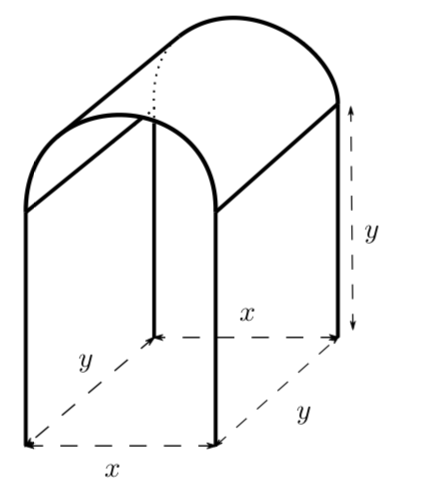
\includegraphics[scale=0.4]{pta.png}
  \end{center}
\end{minipage}
%\end{multicols}

The PTA would like to spend exactly \$5000 on one rain shelter.
\begin{enumerate}[(a)]
\item Write a formula for $y$ in terms of $x$.
\item Find a formula for the total volume in cubic feet covered by the shelter, $V (x)$, if the width of the dashed rectangle has length $x$ feet.
\item The PTA wants to make sure that each of the sides of the rectangle has length at least 5 feet, and the height (that is, $y$) of the shelter is at least 8 feet. In the context of the problem, what is the domain of the function $V (x)$?
\end{enumerate}
\begin{solution}
  See \href{https://dhsp.math.lsa.umich.edu/exams/115exam2/w18/s3.pdf}{https://dhsp.math.lsa.umich.edu/exams/115exam2/w18/s3.pdf}
\end{solution}
\pagebreak
\question (Fall 2017 Exam 2) % problem 3
Jane is designing a water tank using a cone of height $h$ meters and a circular base of radius $r$ meters as shown below.
\begin{center}
  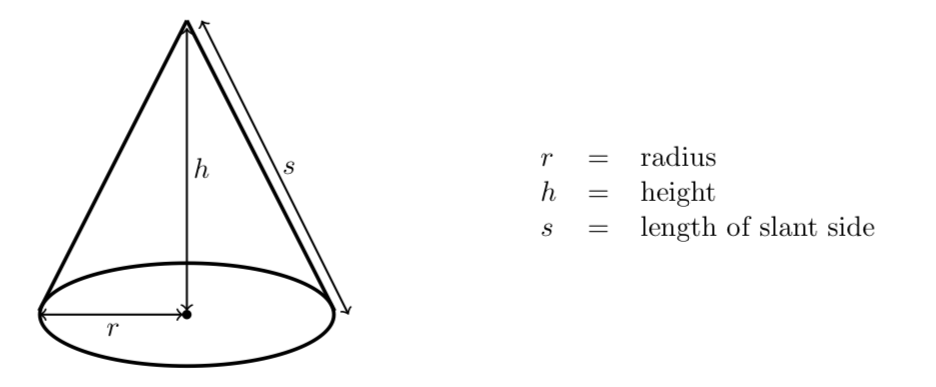
\includegraphics[scale=0.45]{jane.png}
\end{center}
\begin{enumerate}[(a)]
\item The cost of the material for the tank is 3 dollars per square meter for the circular base and 5 dollars per square meter for the cone (without the base). The area, $A$, of the material used for the cone (without the base) is given by the formula $A = \pi rs$ where s is the length of the slant side of the cone, in meters. Find a formula for $s$ in terms of the radius $r$ if Jane plans to spend 200 dollars on the water tank. Your answer should not include the variable $h$.
%\item In the context of this problem, what are appropriate constraints on $r$ and $s$? Circle the one best answer.
%$$0 < r < \infty \qquad 0 < r < s \qquad 0 < r < \sqrt{\frac{200}{3\pi}} \qquad 0 < s < r \qquad 0 < r < \sqrt{\frac{200}{5\pi}}$$
\item Find a formula for $V(r)$, the volume of the tank (in cubic meters) in terms of the radius $r$. Recall that the volume of a cone of radius $R$ and height $H$is $\frac{1}{3} \pi R^2 H$. Your answer should not include the variables $h$ and/or $s$.
\end{enumerate}
\begin{solution}
  See \href{https://dhsp.math.lsa.umich.edu/exams/115exam2/f17/s3.pdf}{https://dhsp.math.lsa.umich.edu/exams/115exam2/f17/s3.pdf}
\end{solution}
\vspace{0.75in}
\question (Winter 2017 Exam 2) % problem 3
  Duncan’s person is making him a new tent in the shape of half a cylinder. She plans to use wire to make the tent frame. This will consist of two semicircles of radius $r$ (measured in inches) attached to three pieces of wire of length $q$ (also measured in inches), as shown in the diagram below. She has 72 inches of wire to use for this.
  \begin{center}
    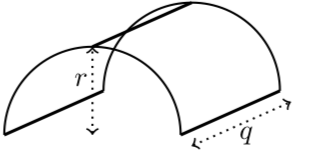
\includegraphics[scale=0.4]{Duncan.png}
  \end{center}
\begin{enumerate}[(a)]
\item Find a formula for $r$ in terms of $q$.
\item Let $V (q)$ be the volume (in cubic inches) of the space inside the tent after the fabric is added, given that the total length of wire is 72 inches and the length of the tent is $q$ inches. (Recall that the tent shape is half of a cylinder.) Find a formula for $V (q)$. The variable r should not appear in your answer.
\item In the context of this problem, what is the domain of $V (q)$?
\end{enumerate}
\begin{solution}
 See \href{https://dhsp.math.lsa.umich.edu/exams/115exam2/w17/s3.pdf}{https://dhsp.math.lsa.umich.edu/exams/115exam2/w17/s3.pdf}
\end{solution}
\end{questions}
\end{document}
%%% Local Variables:
%%% mode: latex
%%% TeX-master: t
%%% End:
